\documentclass{./template/openetcs_report}
\usepackage{color}
%\usepackage[usenames,dvipsnames,svgnames,table]{xcolor}
\usepackage{verbatim,url,lipsum,enumitem}
\usepackage{natbib}
\usepackage{lscape}
\usepackage{longtable}
\usepackage{multirow}
\usepackage{rotating}
\usepackage{graphicx}
\usepackage{amsmath}
\usepackage{rotfloat}
\usepackage{listings}
\lstset{
    breaklines=true, 
    basicstyle=\footnotesize\ttfamily,
    backgroundcolor=\color{white},
    keywordstyle={\color{black}\textbf}, 
    commentstyle=\color{gray}, 
    %stringstyle=\color{nicered}, 
    identifierstyle=\ttfamily, 
    numbers=left, 
    numberstyle=\tiny,
    stepnumber=1,
    xleftmargin=15pt,
    xrightmargin=0pt,
    frame=single,
    framesep=2pt,
    framexleftmargin=0pt,
    framexrightmargin=0pt,
    framextopmargin=0pt,
    framexbottommargin=0pt,
    postbreak=\space, 
    breakindent=5pt, 
    breaklines, 
    showspaces=false, 
    showstringspaces=false
}
\newcommand{\ssection}[1]{\medskip \noindent \textbf{#1.}}

\bibpunct{[}{]}{;}{a}{,}{,}
\parskip 10pt
\graphicspath{{./template/}{.}{./images/}}

\begin{document}


\frontmatter
\project{openETCS}

%Please do not change anything above this line
%============================
% The document metadata is defined below

%assign a report number here
\reportnum{openETCS/WP4/D4.1}

%define your workpackage here
\wp{Work-Package 4: "Requirements for Open Proofs"}

%set a title here
\title{openETCS D4.1: Test Cases Definition -- Draft}

%set a subtitle here
\subtitle{The first draft of definition of test cases}

%set the date of the report here
\date{July 2014}

%define a list of authors and their affiliation here
\author{Huu-Nghia Nguyen}

\affiliation{Institut Telecom}

% define the coverart
\coverart[width=350pt]{chart}

%define the type of report
\reporttype{Preliminary Report}


\begin{abstract}
%define an abstract here
This report presents the first draft of definition of test cases.
Particularly, it defines a format of test cases 
to be later run against API/ Demonstrator.
\end{abstract}

%=============================
%Do not change the next three lines
\maketitle
\tableofcontents
\listoffiguresandtables
%=============================

% The actual document starts below this line
%=============================
\mainmatter

\chapter{Introduction}

The objective of this document is to provide a format to describe test
cases to be later run against API/Demonstrator.

Let's start with the basic definitions. What is a test case?

\begin{itemize}
	\item IEEE Standard Computer Dictionary 610~\cite{Ieee1990} defines a test
	case as
	\begin{quote}
	A set of test inputs, execution conditions, and expected results developed for
	a particular objective, such as to exercise a particular program path or to
	verify compliance with a specific requirement.
	\end{quote}
	
	\item IEEE Standard 829-2008~\cite{Ieee2008} adopted from the definition
	above to define a test case~as
	\begin{quote}
	Documentation specifying inputs, predicted results, and a set of execution
	conditions for a test item.
	\end{quote}

\end{itemize}


The definition of test case format proposed in this document is guided by the
definitions above.
 
%but adding some modifications to adapt to the context of openETCS project.

The rest of the document consists of two chapters. The first chapter describes
a template of test case specifications while the second one give a meta model
using Ecore of the template.

\chapter{Test Case Specification Template}

The purpose of the test cases is to define 
the information needed as it pertains to inputs to and outputs from the 
 being tested. 
A test case specification includes all test case(s) identified by the
associated segment of the level test design (if there is one).
A example of a test case outline is shown below.
Section Introduction is specified once per document. 
The Test Case details in Sections 2 are documented once per Test Case.


\begin{enumerate}
\renewcommand{\labelenumii}{\arabic{enumi}.\arabic{enumii}.}
\item Introduction (once per document)
    \begin{enumerate}
        \item Document identifier 
        \item Document change procedures and history
        \item Glossary
        \item Scope
        \item References
        \item Context
        \item Notation for description
     \end{enumerate}
\item Details (once per test case)
     \begin{enumerate}
        \item Test case identifier 
        \item Objective
        \item Inputs
        \item Outcome(s)
        \item Environmental needs
        \item Special procedural requirements
        \item Intercase dependencies
      \end{enumerate}
\end{enumerate}

\section{Introduction}

Introduce the following subordinate subsections. This section identifies the
issuing organization and the details of issuance. It includes required approvals
and status (DRAFT/FINAL) of the document. It is here that the scope is described
and references identified.

\subsection{Document identifier}
Uniquely identify a version of the document by including information such as the
date of issue, the issuing organization, the author(s), 
and the status/version (e.g., draft, reviewed, corrected, or final). 

It contains basically the following information:
\begin{itemize}
\item Unique "short" name 
\item Version date and version number
\item Organization
\item Author(s)
\item Status 
\end{itemize}

\subsection{Document change procedures and history}
Specify the means for identifying, approving, implementing, and recording
changes to the test case specification. 
This may be recorded in an overall configuration management
system that is documented in a Configuration Management Plan that is referenced
here. 
The change procedures need to include a log of all of the changes that
have occurred since the inception of the MTP. 
This may include a Document ID
(every testing document should have a unique ID connected to the system
project), version number (sequential starting with first approved version),
description of document changes, reason for changes (e.g., audit comments, team
review, system changes), name of person making changes, and role of person to
document (e.g., document author, project manager, system owner). 
This information is commonly put on an early page in the document (after the
title page and before Section 1).

\subsection{Glossary}
Provide an alphabetical list of terms that may require definition for the users
with their corresponding definitions. This includes acronyms. 
There may also be a reference to a project glossary.

\subsection{Scope}
Summarize the software product or system items and features to be tested by this
particular level of test. 
The need for each item and its history may be included.

\subsection{References}
List all of the applicable reference documents. The references are separated
into ``external" references that are imposed external to the project and
``internal" references that are imposed from within to the project.

The external references
list references to the relevant policies or laws that give rise to the need for
this plan, e.g.: a) Laws b) Government regulations c) Standards (e.g.,
governmental and/or consensus) d) Policies. 
The reference to this standard
includes how and if it has been tailored for this project, an overview of the
level(s) of documentation expected, and their contents (or a reference to an
organizational standard or document that delineates the expected test
documentation details).

The internal references list references to documents
such as other plans or task descriptions that supplement this plan, e.g.: a)
Project plan b) Quality assurance plan.


\subsection{Context}
Provide any required context that is not already covered by other sections of
this document (e.g., third- party party testing via the Internet).

\subsection{Notion for description}
Define any numbering schemes, e.g., for scenarios and test cases. The intent of
this section is to explain any such schema.


\section{Details}
\subsection{Test Case Specification Identifier}
Describe the unique identifier needed by each test case so that it can be
distinguished from all other test cases.


\subsection{Objective}

Identify the items or features to be tested by this test case. 
Keep in mind the level for which this test case is written and describe the
items/features accordingly. 
The item description and definition can be referenced from any one
of several sources, depending on the level of the test case specification.
In such a case, it should reference the source document as well.

% \begin{itemize}
% \item Requirements specification 
% \item System Design specification 
% \item Detail Design specification 
% \item Users Guide 
% \item Operations manual
% \item Installation guide 
% \end{itemize}

\subsection{Input Specifications} 

Identify all inputs required to execute the test case. 
Again these may vary based on the level the case is written for. 
Be sure to identify all required inputs not just data elements and values.
Some inputs will be specified by value (with tolerances where appropriate),
whereas others, such as constant tables or transaction files, will be specified
by name. 
Identify all appropriate files, terminal messages, memory
resident areas, and values passed by the operating system.

\begin{itemize}
\item Data 
    \begin{itemize}
    	\item Values 
    	\item Ranges 
    	\item Sets
    \end{itemize} 
\item Table
\item Human actions
\item Conditions 
    \begin{itemize}
    	\item States 
    	\item Initial 
    	\item Intermediate 
    	\item Final
    \end{itemize}
\item Files 
    \begin{itemize}
    	\item Control files 
    	\item Transaction files
    \end{itemize}
\item Relationships 
    \begin{itemize}
        \item Timing 
    \end{itemize}
\end{itemize}

It is also acceptable to simplify the
documentation process by using tables for elements and values. It is even
conceivable to create a test case that can be used a multiple levels of testing
(Unit, Integration, etc.). Notes can be used to document common rules and
processes for elements that have shared characteristics.

Specify all required relationships between inputs (e.g., timing).

% 
% \begin{tabular}{|c|c|c|c|c|c|c|c|c|c|c|}
% \hline
% Case & Test & Valid & Valid & Invalid 
% & R & R & R & ATT & Proc & Dep\\
% Numbers & Element & Values & Response & Response & 1 & 2 & 3 & & &
% \\ \hline
%  & & & & & & & & & &
% \\ \hline
%  & & & & & & & & & &
% \\ \hline
% \end{tabular}
% 
% Where:
% 
% \begin{itemize} 
% 	\item R1 is the valid value rule (i.e. Run one test for each value at
% the beginning and end of the valid set , you should get the valid response) (this
% uses the equivalence partitioning/boundary value technique) 
% 
%     \item R2 is the invalid
% rule (i.e. Run one test for each value just before the beginning and just after
% the end of the valid set , you should get the invalid response) (this uses the
% equivalence partitioning/boundary value technique) 
%     \item R3 is the navigation rule
% between tests ATT is any field specific attributes, (bold, reverse image etc.
%     \item Proc is the procedure to follow for the case. It may be internally
% documented or a separate document 
%     \item Dep are any element or case dependencies 
% \end{itemize}

\subsection{Output Specifications} 

Identify all outputs required to verify the test case.
Again these may vary based on the level the case is written for. 
Be sure to identify all required outputs not just data elements and values.

\begin{itemize}
\item Data 
    \begin{itemize}
        \item Values 
        \item Ranges 
        \item Sets
    \end{itemize} 
\item Tables 
\item Human actions
\item Conditions 
    \begin{itemize}
        \item States 
        \item Initial 
        \item Intermediate 
        \item Final
    \end{itemize}
\item Files 
    \begin{itemize}
        \item Control files 
        \item Transaction files
    \end{itemize}
\item Relationships
\item Timing 
    \begin{itemize}
        \item Response times
        \item Duration 
    \end{itemize}
\end{itemize}

Outputs can also be simplified using tables as noted above
 and may even be included in the same table as the associated input to further
simplify the documentation and improve its usefulness.


\subsection{Environmental needs}

Describe the test environment needed for test setup, execution, and results
recording. This section is commonly documented per scenario or group of
scenarios. It may be illustrated with one or more figures showing all of the
components and where they interact.

\begin{itemize} 
\item  Hardware 
	\begin{itemize}
		\item Configurations 
		\item Limitations
	\end{itemize}
\item Software 
    \begin{itemize}
    	\item Operating systems 
    	\item Compilers 
    	\item Tools 
    	\item Other Application 
    \end{itemize}
\item Other
    \begin{itemize}
    	\item Facilities 
    	\item Training
    \end{itemize}
\end{itemize}


\ssection{Hardware}
Specify the characteristics and configuration(s) of the hardware required to
execute this test case.

\ssection{Software}
Specify all software configuration(s)
required to execute this test case. This may include system software such as
operating systems, compilers, simulators, and test tools. In addition, the test
item may interact with application software.

\ssection{Other}
Specify any other requirements not yet included, e.g., unique facility needs,
specially trained personnel,

\subsection{Special Procedural Requirements}

 Identify any special constraints on
the test case(s). If the test case specification covers more than one test case this
may be the common procedure for several sets of tests or there may be more than
one set of steps or external procedures identified. Focus on key elements such
as:

\begin{itemize}
\item Special Setup 
\item Operations intervention 
\item Output location and identification 
\item Special wrap-up
\end{itemize}

\subsection{Inter-case Dependencies}
 Identify any prerequisite test cases.
It is also recommended that the relationship of test cases be documented at both ends of
the relationship. The precursor should identify any follow-on test cases and the
post cases identify all prerequisites.



% 
% \chapter{Test Cases}
% \section{Formal Definition}
% Basically, a {\em test case} is a sequence of inputs, outputs and durations. 
% It represents a possible trace generated from the SUT.
% 
% \begin{figure}[!htbp]
% \centering
%     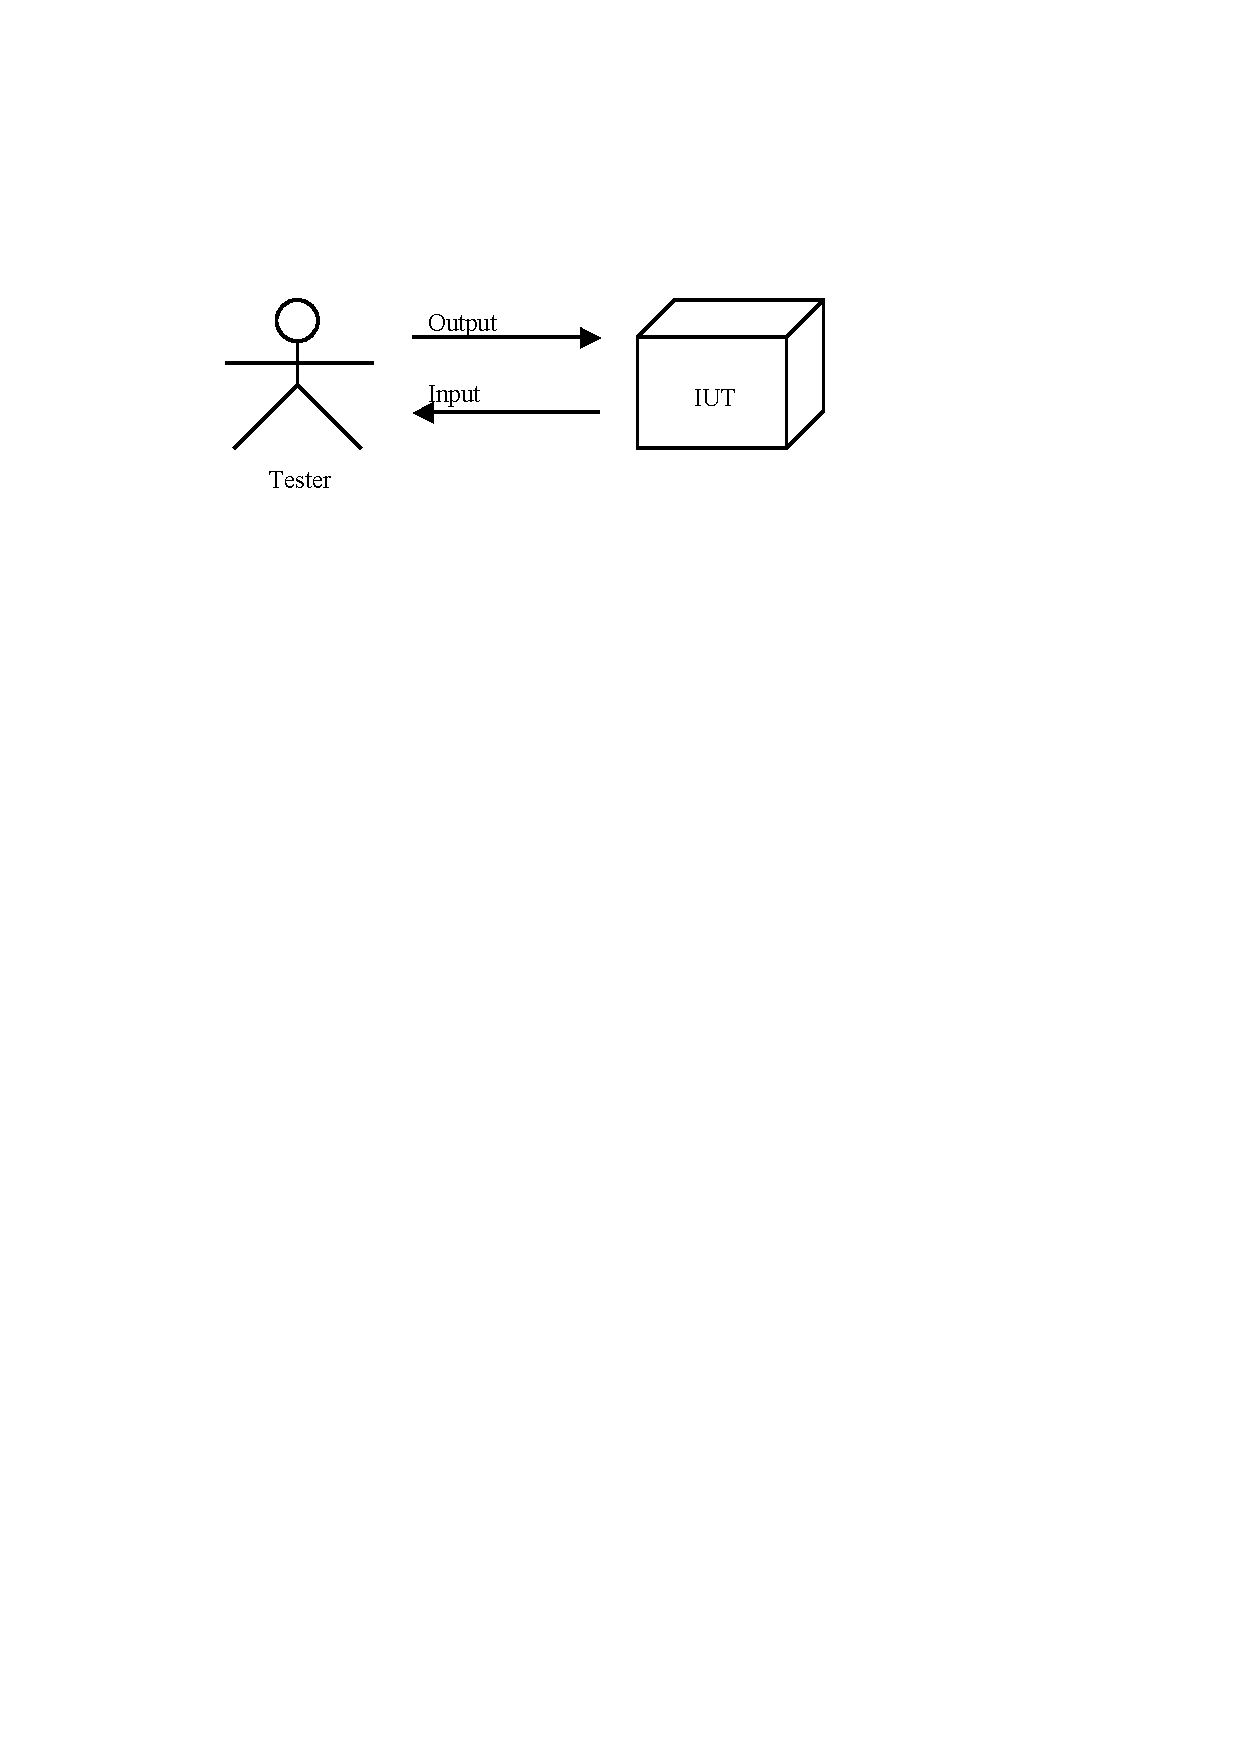
\includegraphics[width=6cm]{images/tester-figure.pdf}
% \label{fig:tester}
% \caption{Basic Events of Testers: Output and Input}
% \end{figure}
% 
% Basically, a  {\em test case} of tester $t$ that test the component $p$ is
% a sequence $\sigma = d_1, \alpha_1, d_2, \alpha_2, \ldots,
% \alpha_m$, where $d_i \in \mathbb{R}$ and each $\alpha_i$ is one of the
% following:
% 
% \begin{itemize}
%     \item $!m(p_1, \ldots, p_n)$: an output of message $m$ 
%     \item $?m(p_1, \ldots, p_n)$: a reception of message $m$ 
% \end{itemize}
% 
% \subsection{Output Specification}
% 
% \subsection{Input Specification}
% 
% \section{Plain Text Format}
% 
% \begin{lstlisting}
% !ETCS_control{}
% delay 4
% ?ETCS_report{{Train}0,10,100,10,start}
% delay 1 
% !ETCS_move{900,105,15}
% delay 4
% ?ETCS_report{{Train}0,10,100,10,moving}
% delay 1
% !ETCS_alarm_to_train{}
% delay 3
% ?ETCS_report{{Train}0,10,100,10,negotiation} 
% \end{lstlisting}


\chapter{Meta Model of Test Cases Specifications}
Ecore Diagram using Eclipse Modeling Framework 

\begin{figure}[!htbp]
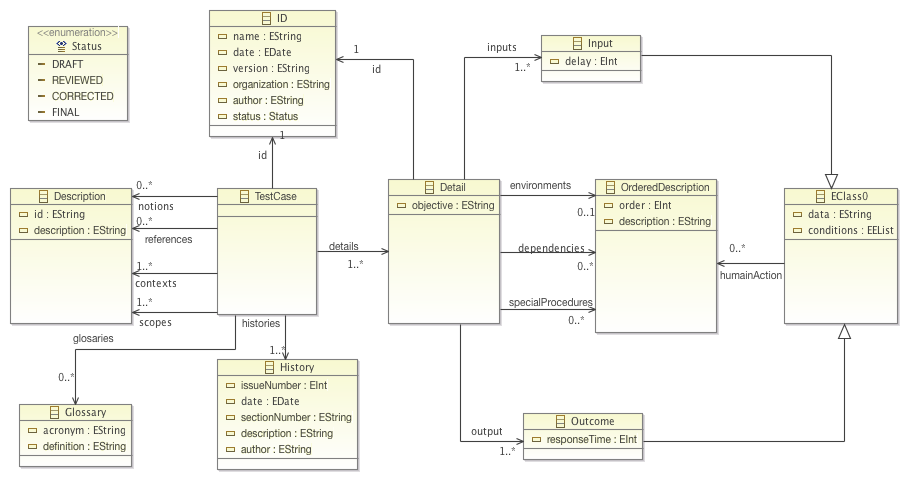
\includegraphics[width=\textwidth]{images/TestMetaModel.png}
\end{figure}

\bibliographystyle{plainnat}
\bibliography{bib}




%===================================================
%Do NOT change anything below this line

\end{document}
